\documentclass{article}
\usepackage[utf8]{inputenc}
\usepackage{amsmath}
\usepackage{float}
\usepackage{listings}
\usepackage[pdftex]{graphicx}
\usepackage{amssymb}
\usepackage{subcaption}
\usepackage{cancel}
\usepackage{float}
\usepackage{hyperref}
\DeclareMathOperator{\sech}{sech}

\newcommand{\pd}[2]{\frac{\partial{#1}}{\partial{#2}}}
%
\newcommand{\pdd}[2]{\frac{\partial^2{#1}}{\partial{#2}^2}}
%
\newcommand{\pddmixed}[3]{\frac{\partial^2{#1}}{\partial{#2}\partial{#3}}}

\newcommand{\grad}[1]{\nabla{#1}}
\newcommand{\deldot}[1]{\nabla \cdot{#1}}
\newcommand{\lap}[1]{\nabla^{2}{#1}}

\newcommand{\bsym}[1]{\boldsymbol{#1}}

\newcommand{\hp}{h^{+}}
\newcommand{\hm}{h^{-}}
%---------------------------------------------------------
\author{Pratik Aghor}
\title{HW $\# 1$: Linear and Energy Stability Theory}
\date{\today}  % Toggle commenting to test

\begin{document}

\maketitle
%----------------------------------------
\section{Thin Liquid Films on a Deformable Substrate:}
%----------------------------------------
Governing equations in dimensionless form:

\begin{align}\label{eq:gov_film_eqns}
 \partial_{t} \hp  + \frac{1}{3}\partial_{x}\left[ (\hp)^{3} (\partial^{3}_{x}\hp + \partial_{x}\kappa) \right] & = 0,\\
 %
 \partial_{t} \hm  + \frac{1}{3}\partial_{x}\left[ (\hm)^{3} (\partial^{3}_{x}\hm - \partial_{x}\kappa) \right] & = 0,\\
 %
 B\partial_{x}^{2}\kappa + [A(1-\Lambda)-2]\kappa & = \partial_{x}^{2}\hp - \partial_{x}^{2}\hm.
\end{align}
Here, $\hp, \hm$ are the thicknesses of the ‘upper’ and ‘lower’ liquid films, respectively, while $\kappa$ is the curvature of the substrrate, which in the small curvature limit is related to the transverse deflection of the substrate $\eta(x, t)$ via the relation $\partial_{x}^{2}\eta = \kappa$ (i.e. $\eta$ is a displacement measured in the direction normal to the ‘horizontal’ x axis). $A$, $B$, and $\Lambda$ are positive external (dimensionless) control parameters related to the axial stiffness, the flexural (bending) stiffness, and the imposed compression of the axial substrate, respectively.
%
The base state is given by $\eta_{B} = \kappa_{B} = 0$ and $\hp_{B} = \hm_{B} = 1$. Perturbing the base state fields and substituting $\phi = \phi_{B} + \phi$, linearizing, we obtain:
\begin{align}\label{eq:linearized_film_eqns}
 \partial_{t} \hp  + \frac{1}{3}\partial_{x}\left[  (\partial^{3}_{x}\hp + \partial_{x}\kappa) \right] & = 0,\\
 %
 \partial_{t} \hm  + \frac{1}{3}\partial_{x}\left[  (\partial^{3}_{x}\hm - \partial_{x}\kappa) \right] & = 0,\\
 %
 B\partial_{x}^{2}\kappa + [A(1-\Lambda)-2]\kappa & = \partial_{x}^{2}\hp - \partial_{x}^{2}\hm.
\end{align}
Substituting the normal mode ansatz $\phi = \phi_{0}e^{\sigma t}e^{i\alpha x} + c.c.$, we get:
\begin{align}
\begin{split}
 \sigma \hp_{0} & = - \frac{1}{3}(i\alpha)^{4}\hp_{0} - \frac{1}{3} (i\alpha)^{2} \kappa_{0}, \\
 %
 \sigma \hm_{0} & = - \frac{1}{3}(i\alpha)^{4}\hm_{0} + \frac{1}{3} (i\alpha)^{2} \kappa_{0}, \\
 %
 B(i\alpha)^{2}\kappa_{0} + [A(1-\Lambda)-2]\kappa_{0} &= (i\alpha)^{2}(\hp_{0} - \hm_{0}).
\end{split}
\end{align}
%
Simplifying,
\begin{align}
\begin{split}
 \sigma \hp_{0} & = - \frac{1}{3}\alpha^{4}\hp_{0} + \frac{1}{3} \alpha^{2} \kappa_{0}, \\
 %
 \sigma \hm_{0} & = - \frac{1}{3}\alpha^{4}\hm_{0} - \frac{1}{3} \alpha^{2} \kappa_{0}, \\
 %
 -B\alpha^{2}\kappa_{0} + [A(1-\Lambda)-2]\kappa_{0} &= -\alpha^{2}(\hp_{0} - \hm_{0}).
\end{split}
\end{align}
%
Subtracting the first two equations,
\begin{equation}
\sigma (\hp_{0} - \hm_{0}) = \frac{1}{3} \{2 \alpha^{2} \kappa_{0} - \alpha^{4}(\hp_{0} - \hm_{0}) \} 
\end{equation}
%
This gives 
\begin{equation}
 (\sigma + \frac{\alpha^{4}}{3})(\hp_{0} - \hm_{0}) = \frac{2}{3}\alpha^{2}\kappa_{0}.
\end{equation}
%
Substituting in the third equation,
\begin{equation}
  -B\alpha^{2}\kappa_{0} + [A(1-\Lambda)-2]\kappa_{0} = -\alpha^{2} \frac{(2/3)\alpha^{2}\kappa_{0}}{(\sigma + \frac{\alpha^{4}}{3})}
\end{equation}
This gives
\begin{equation}\label{eq:thin_film_disp_reln}
 \boxed{ \sigma(\alpha) = -\frac{\alpha^{4}}{3} \left[1 + \frac{2}{([A(1-\Lambda)-2] - B\alpha^{2})} \right] }. 
\end{equation}
If $[A(1-\Lambda)-2] \ll B\alpha^{2}$, it is the Type-IIs instability. 
\begin{figure}[H]
    \centering
    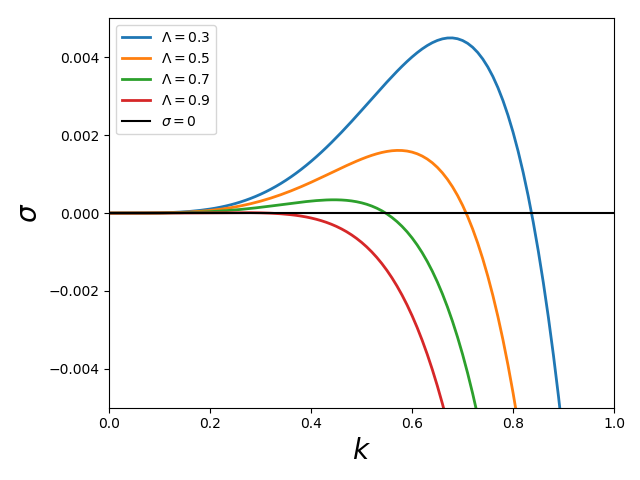
\includegraphics[scale = 0.5]{Figs/thin_liq_films_deformable_substrate_dispersion_reln.png}
    \caption{As $\Lambda$ decreases, we see a Type-IIs type instability. Here, $A = B = 0.5$.}
    \label{fig:thin_liq_films_deformable_substrate_dispersion_reln}
\end{figure}
For marginal stability curve, we substitute $\sigma = 0$ in Eqn.(\ref{eq:thin_film_disp_reln}).
%
This yields:
\begin{equation}\label{eq:thin_film_marginal_stab}
 \frac{[A(1-\Lambda)]}{B} = \alpha^{2}
\end{equation}
Assuming $\Lambda$ to be our control parameter,
\begin{equation}
 \Lambda = 1 - B\alpha^{2}/A
\end{equation}
\begin{figure}[H]
    \centering
    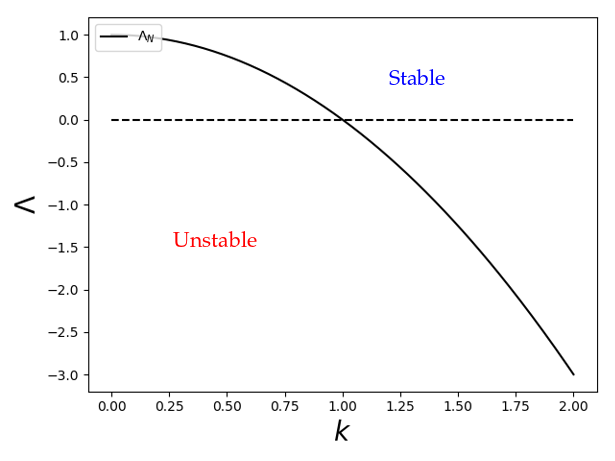
\includegraphics[scale = 0.4]{Figs/thin_liq_films_deformable_substrate_marginal_stab.png}
    \caption{Marginal stability curve. Here, $A = B = 0.5$.}
    \label{fig:thin_liq_films_deformable_substrate_marginal_stab}
\end{figure}
Fastest growing mode can be found by finding where $\pd{\sigma}{\alpha} = 0$. However, since $\sigma \equiv \sigma (\alpha^{2})$, we can equivalently find $\pd{\sigma}{(\alpha^{2})} = 0$ to find the fastest growing mode. We represent $[A(1-\Lambda)-2] \equiv \# $ for simplicity. 
\begin{align}
 \begin{split}
  \pd{\sigma}{(\alpha^{2})} &= \frac{-2\alpha^{2}}{3} - \frac{2}{3}\frac{\left[ (\# - B\alpha^{2})(2\alpha^{2})- \alpha^{4}(-B)\right]}{(\# - B\alpha^{2})^{2}} \\
  %
  0 & = -\alpha^{2} - \frac{-B\alpha^{4} + 2 \# \alpha^{2}}{(\# - B\alpha^{2})^{2}} \\
  %
  0 & = -1 + \frac{B\alpha^{2} - 2\#}{(\# - B\alpha^{2})^{2}}\\
  %
  (\# - B\alpha^{2})^{2} & = B\alpha^{2} - 2\# \\
  %
  \#^{2} + B^{2}\alpha^{4} - 2\# B \alpha^{2} &= B\alpha^{2} - 2\# \\
  %
  0 & = B^{2}\alpha^{4} - (2\# + 1) B \alpha^{2} +(\#^{2} + 2\#)\\
  %
  \alpha^{2} &= \frac{(2\# + 1) \pm \sqrt{(1- 4 \#)} }{2B}\\
  \end{split}
\end{align}
Therefore, the fastest growing modes will be
$\boxed{\alpha_{f} = \pm \sqrt{\frac{(2\# + 1) \pm \sqrt{(1- 4 \#)} }{2B}} }$. (Have to check which of the inner $\pm$ modes will be fastest. Can be done by substituting into the dispersion relation and varying parameters.)
%----------------------------------------
\section{$2D$ pattern forming system (one confined direction): Two-component porous medium convection:}
%----------------------------------------
2D convection in a fluid-saturated porous layer confined between plane parallel rigid boundaries coincident with $z = 0$ and $z = 1$ but now with two (dimensionless) scalar fields, namely the temperature $T (x, z, t)$ and the salt concentration $S(x, z, t)$, that
determine the density of the fluid.

\begin{align}
 \begin{split}
  \deldot{\bsym{u}} &= 0, \\
  %
  \bsym{u} & = -\grad{P} + (Ra_{T}T - Ra_{S}S)\bsym{\hat{e}_{z}},\\
  %
  \partial_{t}T + \bsym{u}\cdot\grad{T} &= \lap{T},\\
  %
  \partial_{t}S + \bsym{u}\cdot\grad{S} &= \tau\lap{S}.\\
 \end{split}
\end{align}
where $Ra_{T}$ and $Ra_{S}$ are thermal and solutal Rayleigh numbers and $0 < \tau < 1$ is the diffusivity ratio. We define a streamfunction $\psi$ such that $u = \partial_{z}\psi$ and $w = - \partial_{x}\psi$. Eliminating pressure by taking the curl of the Darcy's law (momentum equation) and taking the $y$ component, we obtain:
\begin{align}
 \begin{split}
  \cancel{-}\left[\pd{w}{x} - \pd{u}{z}\right] &= \cancel{-} \pd{}{x}\left[Ra_{T}T - Ra_{S}S\right]\\
  %
  -\psi_{xx} - \psi_{zz} &= Ra_{T} T_{x} - Ra_{S} S_{x}, \\
  %
  \Rightarrow \lap{\psi} &= Ra_{S}S_{x} - Ra_{T}T_{x}.
 \end{split}
\end{align}

%----------------------------------------
\subsection{Linear Stability Analysis:}
%----------------------------------------
Base state $T_{B} (z) = C_{B}(z) = 1 - z$ and $\psi_{B} = 0$. Substituting $T = T_{B} + \theta$,$S = C_{B} + c$, $\psi = \psi_{B} + \psi$ and linearizing, obtain:
\begin{align}
 \begin{split}
  \psi_{xx} + \psi_{zz} &= Ra_{S}S_{x} - Ra_{T}\theta_{x}\\
  %
  \partial_{t}\theta - \psi_{x}(-1) &= \theta_{xx} + \theta_{zz}\\
  %
  \partial_{t}c - \psi_{x}(-1) &= c_{xx} + c_{zz}\\
 \end{split}
\end{align}
%
\begin{align}
 \begin{split}
  \psi_{xx} + \psi_{zz} + (Ra_{T}\theta_{x} - Ra_{S}c_{x}) &= 0  \\
  %
  - \psi_{x} + \theta_{xx} + \theta_{zz} &= \partial_{t}\theta\\
  %
  - \psi_{x} + c_{xx} + c_{zz} &= \partial_{t}c \\
 \end{split}
\end{align}
Substituting the normal mode ansatz $\phi = \hat{\phi}(z) e^{ikx} + \textrm{c.c.}$, where c.c. is the complex conjugate, we obtain the following linear eigenvalue problem:

\begin{equation}
 \begin{bmatrix}
  D^{2} - k^{2} & (ik) Ra_{T} & -(ik)Ra_{S}\\
  %
  -(ik) & D^{2} - k^{2} & 0 \\
  %
  -(ik) & 0 & \tau(D^{2} - k^{2})
 \end{bmatrix}
 %
 \begin{bmatrix}
  \hat{\psi}\\
  \hat{\theta}\\
  \hat{c}
 \end{bmatrix}
 = \sigma \begin{bmatrix}
           0 & 0 & 0\\
           0 & 1 & 0\\
           0 & 0 & 1
          \end{bmatrix}
%
 \begin{bmatrix}
  \hat{\psi}\\
  \hat{\theta}\\
  \hat{c}
 \end{bmatrix}
\end{equation}
However, for this particular problem, we can do better than this. We have Dirichlet BC's on $\theta$, $c$ and $w$, i.e., $\theta = c = \partial_{x}\psi = 0 $ at $z = 0, 1$. The last condition, however, can be interpreted as follows: At the boundaries ($z = 0, 1$), $\psi$ is constant in $x$. Since $\psi$ is independent of $x$, we can set the value of $\psi = 0$ at the boundaries, without loss of generality. Anyway, we are interested in the velocity fields and those can be obtained from the derivatives of $\psi$, not $\psi$ itself. Hence, the boundary conditions can be taken to be $\theta = c = \psi = 0 $ at $z = 0, 1$. With this information, we can guess the $z$-dependence of the perturbation fields to be $\sim \sin(m\pi z)$. Writing $\hat{\phi} = \phi_{0} \sin(m\pi z)$, we further simplify the above system as:
\begin{equation}\label{eq:eigenproblem}
 \begin{bmatrix}
  -(k^{2} + m^{2}\pi^{2}) & (ik) Ra_{T} & -(ik)Ra_{S}\\
  %
  -(ik) & -(k^{2} + m^{2}\pi^{2}) & 0 \\
  %
  -(ik) & 0 & -\tau(k^{2} + m^{2}\pi^{2})
 \end{bmatrix}
 %
 \begin{bmatrix}
  \psi_{0}\\
  \theta_{0}\\
  c_{0}
 \end{bmatrix}
 = \sigma \begin{bmatrix}
           0 & 0 & 0\\
           0 & 1 & 0\\
           0 & 0 & 1
          \end{bmatrix}
%
 \begin{bmatrix}
  \psi_{0}\\
  \theta_{0}\\
  c_{0}
 \end{bmatrix}
\end{equation}
We can solve this system analytically for each $k$, yielding a quadratic in $\sigma$, giving two roots for each $k$. However, I found the expression to be too cumbersome and resorted to numerics at this point. For $Ra_{S} = \tau = 0$, I was able to recover the dispersion relation for the one-component porous medium convection that we derived in class, with $k_{c} = \pi$ and $Ra_{Tc} = 4\pi^{2}$.  

\begin{figure}[H]
    \centering
    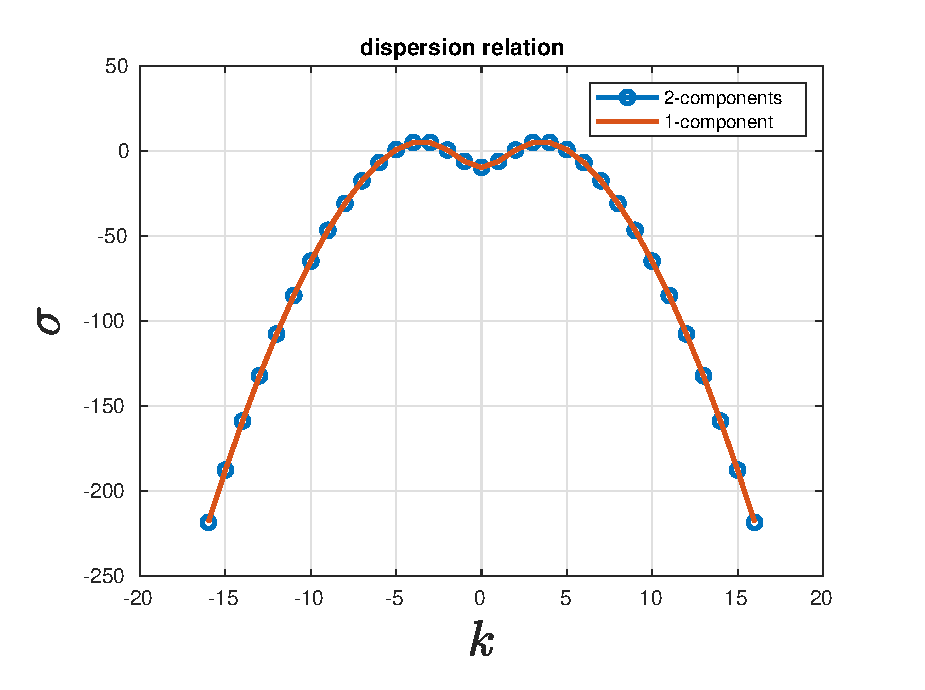
\includegraphics[scale = 0.8]{Figs/sigma_vs_k_comparison.eps}
    \caption{Comparison between dispersion relations obtained for $Ra_{S} = \tau = 0$ ($2$-components) and for the one-component porous medium convection. $Ra_{T} = 4\pi^{2} + 10$.}
    \label{fig:sigma_vs_k_comparison}
\end{figure}
%
For marginal stability we substitute $\sigma = 0$ and the condition for marginal stability then becomes $\textrm{det}(A) = 0$, where $A$ is the LHS matrix in Eqn.(\ref{eq:eigenproblem}). It is easy to calculate the determinant using third row and expansion in minors.  
\begin{equation}\label{eq:lin_marginal_stab}
 k^{2}(\tau Ra_{T} - Ra_{S}) = \tau (k^{2} + m^{2}\pi^{2})^{2}.
\end{equation}

%----------------------------------------
\subsection{Energy Stability Analysis:}
%----------------------------------------
To perform energy stability analysis, we first need to create an energy-like quantity. We do not linearize equations at any point and deal with full nonlinear evolution equations in this approach. Multiplying $\theta$-equation by $\theta$, $c$-equation by $c$ and adding them, we create a quadratic, positive definite energy-like quantity. Let us first focus on the $\theta$-equation.
\begin{align}
 \begin{split}
  & \int_{0}^{1} \int_{0}^{L_{x}}\theta \left[\partial_{t}\theta + \bsym{u}.\grad{\theta} = w + \lap{\theta}\right] dx dz \\
  %
  &\int_{0}^{1} \int_{0}^{L_{x}}\theta \left[\partial_{t}\theta + \deldot{\left(\bsym{u} \frac{\theta^{2}}{2}\right)}- \frac{\theta^{2}}{2}\cancelto{0}{\deldot{\bsym{u}}} = w + \lap{\theta}\right] dx dz \\
  %
  &\textrm{NOTE:} \deldot{\left(\bsym{u} \frac{\theta^{2}}{2}\right)} = \int_{0}^{1}\cancelto{0 \because \textrm{periodic BCs} }{\left[\int_{0}^{L_{x}} \partial_{x}(u\theta^{2}/2) dx\right]}dz + \int_{0}^{L_{x}}\cancelto{0 \because \textrm{z-BCs}}{\left[\int_{0}^{1} \partial_{z}(w\theta^{2}/2) dz \right]}dx\\
  %
  & \partial_{t}\left[\int_{0}^{1} \int_{0}^{L_{x}} \frac{\theta^{2}}{2} dx dz\right] = \int_{0}^{1} \int_{0}^{L_{x}}\left[w\theta  + \theta \lap{\theta} \right] dx dz\\
  %
  &\textrm{using integration by parts (IBP) and BCs} \hdots\\
  %
  &\partial_{t}\left[\int_{0}^{1} \int_{0}^{L_{x}} \frac{\theta^{2}}{2} dx dz\right] = \int_{0}^{1} \int_{0}^{L_{x}}\left[w\theta  + \cancelto{0 \because \theta = 0 \textrm{ at } z=0, 1}{\deldot{\theta \grad{\theta}}} - |\grad{\theta}|^{2} \right]dx dz\\
  %
  &\partial_{t}\left[\int_{0}^{1} \int_{0}^{L_{x}} \frac{\theta^{2}}{2} dx dz\right] = \int_{0}^{1} \int_{0}^{L_{x}}\left[w\theta  - |\grad{\theta}|^{2} \right]dx dz\\
 \end{split}
\end{align}
Similarly, we can obtain another equation by multiplying $c$ to the $c$-equation and integrating over the domain. 
\begin{equation}
 \partial_{t}\left[\int_{0}^{1} \int_{0}^{L_{x}} \frac{c^{2}}{2} dx dz\right] = \int_{0}^{1} \int_{0}^{L_{x}}\left[wc  - \tau |\grad{c}|^{2} \right]dx dz
\end{equation}
%
Adding these two equations and defining $\boxed{E(t) = \int_{0}^{1} \int_{0}^{L_{x}} \left[ \frac{\tilde{\theta}^{2}}{2} + \frac{\tilde{c}^{2}}{2} \right] dx dz } $, we obtain:
\begin{equation}\label{eq:energy-stab-formulation}
 \frac{dE}{dt} =  \int_{0}^{1} \int_{0}^{L_{x}}\left[ \tilde{w} (\tilde{\theta} + \tilde{c})   - |\grad{\tilde{\theta}}|^{2} - \tau |\grad{\tilde{c}}|^{2} \right]dx dz
\end{equation}
We define a quantity $\lambda = \textrm{min} \{ \int_{0}^{1} \int_{0}^{L_{x}} \left[|\grad{\tilde{\theta}}|^{2} + \tau |\grad{\tilde{c}}|^{2} - \tilde{w} (\tilde{\theta}+ \tilde{c}) \right] dxdz\}$, where $\tilde{w}$ is slaved to $\tilde{\theta}, \tilde{c}$ in the same way as $w$ is slaved to $\theta$ and $c$, i.e. $\lap{w} = -Ra_{s} c_{xx} + Ra_{T} \theta_{xx}$ or $w = \mathcal{L}(\theta, c)$. If we can prove $\lambda > 0$, this would imply $dE/dt < 0$ and that the system is energy stable. 
%----------------------------------------
\subsubsection{Variational Formulation:}
%----------------------------------------
Let 
%
\begin{equation}
 J[\tilde{\theta}, \tilde{c}] = \int_{0}^{1} \int_{0}^{L_{x}} \left[|\grad{\tilde{\theta}}|^{2} + \tau |\grad{\tilde{c}}|^{2} - \tilde{w} (\tilde{\theta} + \tilde{c}) \right] dxdz
\end{equation}
%
, such that $\tilde{w} = \mathcal{L}(\tilde{\theta}, \tilde{c})$. Also, we impose a normalization constraint on the energy-like quantity to keep book-keeping simple (The idea of normalizing is similar to matrix norms $||A|| = \max_{x\neq 0} \frac{||Ax||}{||x||} = \max_{x \neq 0, ||x|| = 1} ||Ax||$ ). We demand, $\int_{0}^{1} \int_{0}^{L_{x}} \left[ \frac{\tilde{\theta}^{2}}{2} + \frac{\tilde{c}^{2}}{2} \right] dx dz  = 1$. We now have a variational problem at hand, with the `cost functional' $J(\tilde{\theta}, \tilde{c})$ (to be minimized) subject to constraints $\tilde{w} = \mathcal{L}(\tilde{\theta}, \tilde{c})$ and $\int_{0}^{1} \int_{0}^{L_{x}} \left[ \frac{\tilde{\theta}^{2}}{2} + \frac{\tilde{c}^{2}}{2} \right] dx dz  = 1$. This leads us to define the Lagrangian/ Lagrange functional $L$:
\begin{align}
 \begin{split}
   L(\tilde{\theta}, \tilde{c}, \tilde{w}, v, \Lambda)  &\equiv  \int_{0}^{1} \int_{0}^{L_{x}} \left[|\grad{\tilde{\theta}}|^{2} + \tau |\grad{\tilde{c}}|^{2} - \tilde{w} (\tilde{\theta}+ \tilde{c}) \right] dxdz \\
   %
   &- \int_{0}^{1} \int_{0}^{L_{x}} v (\lap{\tilde{w}} + Ra_{s} c_{xx} - Ra_{T} \theta_{xx} ) dxdz \\
   %
   &- \Lambda \left[\int_{0}^{1} \int_{0}^{L_{x}}  \frac{\tilde{\theta}^{2}}{2} + \frac{\tilde{c}^{2}}{2}  dx dz - 1\right],   
 \end{split}
\end{align}
where $v$ is a Lagrange multiplier field and $\Lambda$ is a scalar Lagrange multiplier. 
%
Now, we must set the first variations of $L$ with respect to each of its arguments. We start with $\frac{\delta L}{\delta \tilde{\theta}} = 0$. From variational calculus, we know this is equivalent to $\left. \frac{d}{d\epsilon}L(\tilde{\theta} + \epsilon \eta, \tilde{c}, \tilde{w}, v, \Lambda)\right|_{\epsilon = 0} = 0$, with $\eta$ satisfying $\eta = 0$ at $z = 0, 1$. 

\begin{align}
 \begin{split}
  L(\tilde{\theta} + \epsilon \eta, \tilde{c}, \tilde{w}, v, \Lambda) & = \int_{0}^{1} \int_{0}^{L_{x}} \left[|\grad{\tilde{\theta}} + \epsilon \eta|^{2} + \tau |\grad{\tilde{c}}|^{2} - \tilde{w} (\tilde{\theta} + \epsilon \eta + \tilde{c}) \right] dxdz \\
   %
   &- \int_{0}^{1} \int_{0}^{L_{x}} v (\lap{\tilde{w}} + Ra_{s} c_{xx} - Ra_{T} \theta_{xx} - \epsilon Ra_{T} \eta_{xx} ) dxdz \\
   %
   &- \Lambda \left[\int_{0}^{1} \int_{0}^{L_{x}}  \left(\frac{(\tilde{\theta} +\epsilon \eta)^{2}}{2} + \frac{\tilde{c}^{2}}{2}  \right) dx dz - 1\right] ,\\ 
   %
   & = \int_{0}^{1} \int_{0}^{L_{x}} \left[|\grad{\tilde{\theta}}|^{2} + 2\epsilon \grad{\tilde{\theta}}\cdot \grad{\eta} + \epsilon^{2}|\grad{\eta}|^{2} +\tau |\grad{\tilde{c}}|^{2}  - \tilde{w} (\tilde{\theta} + \epsilon \eta + \tilde{c}) \right] dxdz \\
   %
   &- \int_{0}^{1} \int_{0}^{L_{x}} v (\lap{\tilde{w}} + Ra_{s} c_{xx} - Ra_{T} \theta_{xx} - \epsilon Ra_{T} \eta_{xx} ) dxdz \\
   %
   &- \Lambda \left[\int_{0}^{1} \int_{0}^{L_{x}}  \left(\frac{\tilde{\theta}^{2} +2\epsilon \tilde{\theta}\eta + \epsilon^{2}\eta^{2})}{2} + \frac{\tilde{c}^{2}}{2}  \right) dx dz - 1\right]
 \end{split}
\end{align}
%
Taking the first derivative of the above expression wrt $\epsilon$ and evaluating at $\epsilon = 0$, we get:
\begin{align}
 \begin{split}
  \frac{\delta L}{\delta \tilde{\theta}} & = \int_{0}^{1} \int_{0}^{L_{x}} \left[2 \grad{\tilde{\theta}}\cdot \grad{\eta} - \tilde{w} \eta \right] dxdz \\
   %
   &- \int_{0}^{1} \int_{0}^{L_{x}} v (-Ra_{T} \eta_{xx} ) dxdz \\
   %
   &- \Lambda \left[\int_{0}^{1} \int_{0}^{L_{x}} \tilde{\theta}\eta  dx dz \right], \\
   %
   0 & = \int_{0}^{1} \int_{0}^{L_{x}}\left[2\grad{\tilde{\theta}} \cdot \grad{\eta} - \tilde{w}\eta + Ra_{T} v \eta_{xx} - \Lambda \tilde{\theta}\eta \right]\\
   %
 \end{split}
\end{align}
We want everything to be proportional to $\eta$, so using IBP to factor out $\eta$ from each term - For example,
\begin{align}
 \begin{split}
 \int_{0}^{1} \int_{0}^{L_{x}}2\grad{\tilde{\theta}} \cdot \grad{\eta} dxdz & = \int_{0}^{1} \int_{0}^{L_{x}} 2 \deldot{\eta \grad{\tilde{\theta}}} - 2 \eta \lap{\tilde{\theta}} dx dz\\
 %
 & = \int_{0}^{1}\cancelto{0}{\left(\int_{0}^{L_{x}}\partial_{x}[\eta \partial_{x}\tilde{\theta}] dx \right) }dz + \int_{0}^{Lx} \cancelto{0}{\left(\int_{0}^{1}\partial_{z}[\eta \partial_{z}\tilde{\theta}] dz\right)} dx \\
 & - \int_{0}^{1} \int_{0}^{L_{x}}2 \eta \lap{\tilde{\theta}} dx dz, 
  \end{split}
\end{align}
Both the boundary terms vanish since $\eta (0) = \eta(1) = 0$ in $z$ and periodic BCs in $x$. Similarly for other terms, we obtain
\begin{equation}
 0 = \int_{0}^{1} \int_{0}^{L_{x}}\eta \left[-2\lap{\tilde{\theta}} - \tilde{w} + Ra_{T} \partial_{xx} v  - \Lambda \tilde{\theta} \right]dxdz.
\end{equation}
Since this must be true for all $\eta$ (satisfying appropriate BCs), we must have
\begin{equation}
 \boxed{-2\lap{\tilde{\theta}} - \tilde{w} + Ra_{T} \partial_{xx} v = \Lambda \tilde{\theta}}.
\end{equation}
%
Similarly, setting variation of $L$ wrt $\tilde{c}$ to be zero ($\frac{\delta L}{\delta \tilde{c}} = 0$), we get
\begin{equation}
 \boxed{-2\tau \lap{\tilde{c}} - \tilde{w} - Ra_{S} \partial_{xx} \tilde{v} = \Lambda \tilde{c}}.
\end{equation}
%
$\frac{\delta L}{\delta \tilde{w}} = 0$ gives
\begin{equation}
 \boxed{\lap{\tilde{v}} + \tilde{\theta} + \tilde{c} = 0}.
\end{equation}
%
$\frac{\delta L}{\delta \tilde{v}} = 0$ gives
\begin{equation}
 \boxed{\lap{\tilde{w}} + (Ra_{S}\tilde{c}_{xx} - Ra_{T}\tilde{\theta}_{xx}) = 0. } 
\end{equation}
And finally, $\frac{\delta L}{\delta \Lambda} = 0$ gives back the normalization condition. 
%----------------------------------------
Substituting $\tilde{\phi} = \phi_{E} \sin({m\pi z}) e^{ikx}$, we get:
\begin{align}
 \begin{split}
  & 2 (m^{2}\pi^{2} + k^{2}) \theta_{E} - w_{E} - k^{2}Ra_{T} v_{E} = \Lambda \theta_{E}, \\
  %
  & 2 \tau (m^{2}\pi^{2} + k^{2}) c_{E} - w_{E} + k^{2}Ra_{S} v_{E} = \Lambda c_{E}, \\
  %
  & -(m^{2}\pi^{2} + k^{2}) v_{E} + \theta_{E} + c_{E} = 0,\\
  %
  &-(m^{2}\pi^{2} + k^{2}) w_{E} + k^{2}(Ra_{T} \theta_{E} - Ra_{S}c_{E}) = 0.
 \end{split}
\end{align}
Multiplying the first two equations by $(m^{2}\pi^{2} + k^{2})$ and substituting the third and fourth equations into them, we get
\begin{align}
 \begin{split}
  & 2 (m^{2}\pi^{2} + k^{2})^{2} \theta_{E} - k^{2}(Ra_{T} \theta_{E} - Ra_{S}c_{E}) - k^{2}Ra_{T} (\theta_{E} + c_{E}) = \Lambda (m^{2}\pi^{2} + k^{2}) \theta_{E}, \\
  %
  & 2 \tau (m^{2}\pi^{2} + k^{2})^{2} c_{E} - k^{2}(Ra_{T} \theta_{E} - Ra_{S}c_{E}) + k^{2}Ra_{S} (\theta_{E} + c_{E}) = \Lambda (m^{2}\pi^{2} + k^{2}) c_{E}. \\
  %
 \end{split}
\end{align}
Separating coefficients of $\theta_{E}, c_{E}$, get:
\begin{align}
 \begin{split}
  [2 (m^{2}\pi^{2} + k^{2})^{2} - 2k^{2}Ra_{T}] \theta_{E} + k^{2}(Ra_S - Ra_T) c_{E} &= \Lambda (m^{2}\pi^{2} + k^{2}) \theta_{E},\\
  %
  k^{2}(Ra_S - Ra_T)\theta_{E} + [2 \tau (m^{2}\pi^{2} + k^{2})^{2} + 2k^{2}Ra_{S}] c_{E} &= \Lambda (m^{2}\pi^{2} + k^{2}) c_{E}.
 \end{split}
\end{align}
Writing into a matrix-form
\begin{equation}
 \begin{bmatrix}
  (2 (m^{2}\pi^{2} + k^{2})^{2} - 2k^{2}Ra_{T}) & k^{2}(Ra_S - Ra_T)\\
  %
  k^{2}(Ra_S - Ra_T) & (2 \tau (m^{2}\pi^{2} + k^{2})^{2} + 2k^{2}Ra_{S})
 \end{bmatrix}
 %
 \begin{bmatrix}
  \theta_{E}\\
  c_{E}
 \end{bmatrix}
 = \Lambda (m^{2}\pi^{2} + k^{2})\begin{bmatrix}
  \theta_{E}\\
  c_{E}
 \end{bmatrix}.
\end{equation}
For energy stability, want $\Lambda > 0$, Minimum $\Lambda = 0$. To get the marginal energy-stability curve, we solve for $\Lambda = 0$. The determinant of the LHS matrix must vanish for $Ax = 0$ to have a nontrivial solution. Hence, the condition becomes:
\begin{align}\label{eq:energy_marginal_stab}
\begin{split}
 & 4\tau (m^{2}\pi^{2} + k^{2})^{4} + 4 k^{2}Ra_{S} (m^{2}\pi^{2} + k^{2})^{2} - 4\tau k^{2} Ra_{T} (m^{2}\pi^{2} + k^{2})^{2} - 4 k^{4} Ra_{T}Ra_{S} \\
 & - k^{4}(Ra_{S}^{2} + Ra_{T}^{2} - 2 Ra_{T}Ra_{S}) = 0,\\
 %
 \Rightarrow &4\tau (m^{2}\pi^{2} + k^{2})^{4} + 4 k^{2}Ra_{S} (m^{2}\pi^{2} + k^{2})^{2} - 4\tau k^{2} Ra_{T} (m^{2}\pi^{2} + k^{2})^{2}\\
 %
 &- 2 k^{4} Ra_{T}Ra_{S} - k^{4}(Ra_{S}^{2} + Ra_{T}^{2}) = 0, \\
 %
 \Rightarrow & \boxed{4\tau (m^{2}\pi^{2} + k^{2})^{4} + 4 k^{2}(m^{2}\pi^{2} + k^{2})^{2}(Ra_{S} - \tau Ra_{T} ) - k^{4}(Ra_{S} + Ra_{T})^{2} = 0}.
\end{split}
\end{align}
%
\begin{figure}[H]
\centering
\begin{subfigure}{0.49\textwidth}
  \centering
  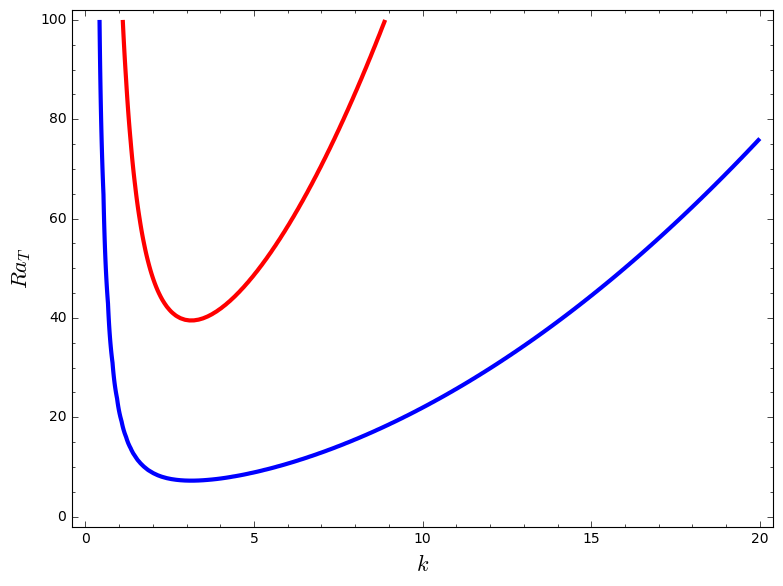
\includegraphics[scale=0.3]{Figs/energy_stab_Ra_T_vs_k_Ra_S_0_01_tau_0_01.png}
 \subcaption{}
  \label{fig:energy_stab_Ra_T_vs_k_Ra_S_0_01_tau_0_01}
\end{subfigure}%
\begin{subfigure}{.49\textwidth}
  \centering
  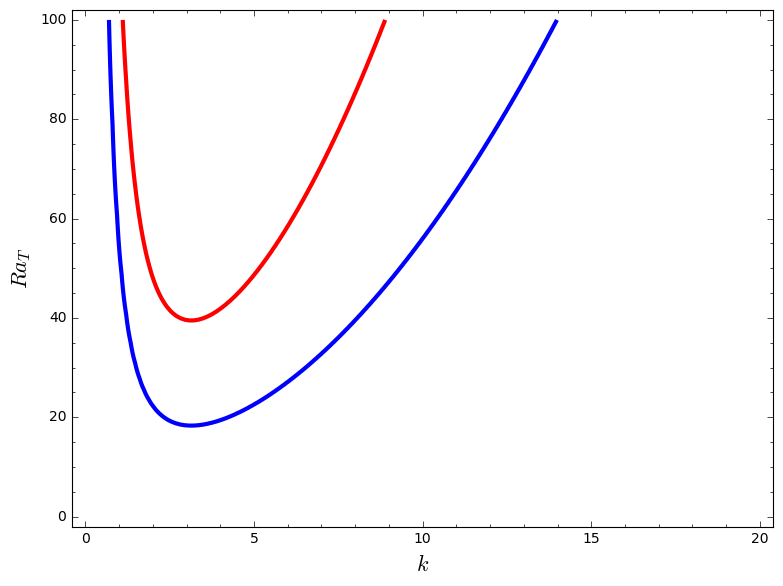
\includegraphics[scale=0.3]{Figs/energy_stab_Ra_T_vs_k_Ra_S_0_01_tau_0_1.png}
  \subcaption{}
  \label{fig:energy_stab_Ra_T_vs_k_Ra_S_0_01_tau_0_1}
    \end{subfigure}
    \begin{subfigure}{.49\textwidth}
  \centering
  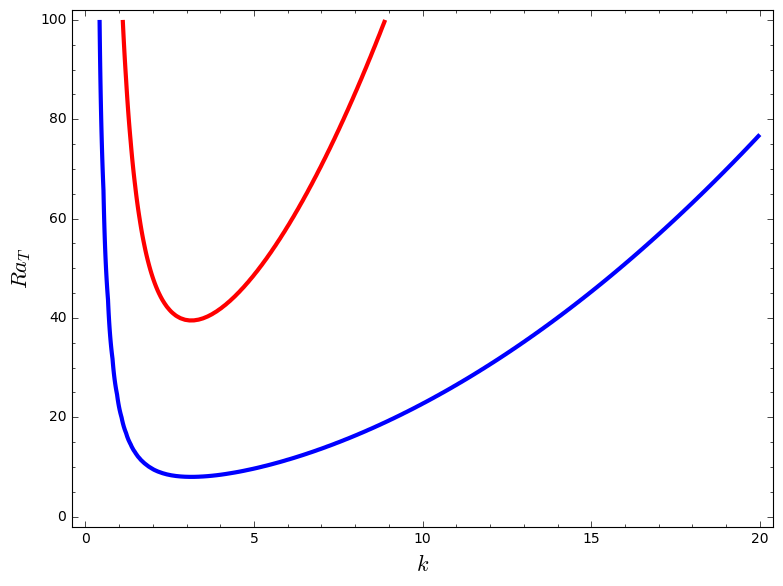
\includegraphics[scale=0.3]{Figs/energy_stab_Ra_T_vs_k_Ra_S_0_1_tau_0_01.png}
  \subcaption{}
  \label{fig:energy_stab_Ra_T_vs_k_Ra_S_0_1_tau_0_01}
    \end{subfigure}
        \begin{subfigure}{.49\textwidth}
  \centering
  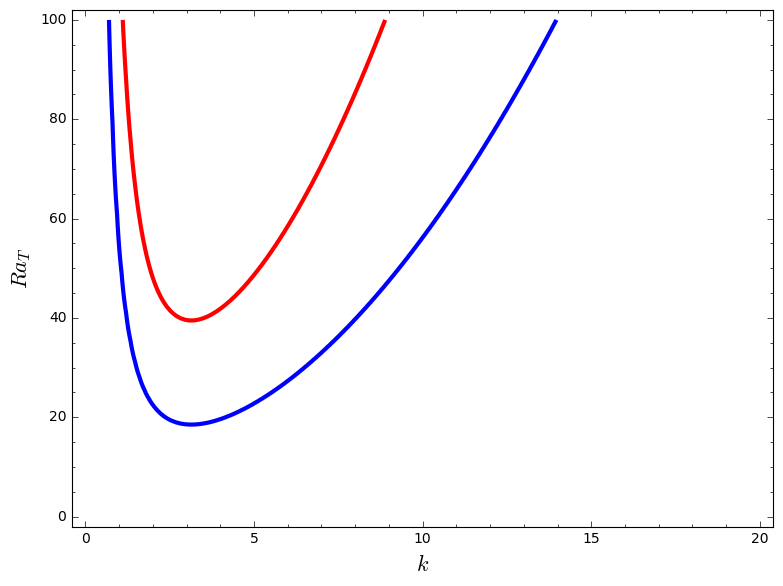
\includegraphics[scale=0.3]{Figs/energy_stab_Ra_T_vs_k_Ra_S_0_1_tau_0_1.png}
  \subcaption{}
  \label{fig:energy_stab_Ra_T_vs_k_Ra_S_0_1_tau_0_1}
    \end{subfigure}
  \caption{(a) $Ra_{S} = 10^{-2}, \tau = 10^{-2}$, (b)$Ra_{S} = 10^{-2}, \tau = 10^{-1}$, (c) $Ra_{S} = 10^{-1}, \tau = 10^{-2}$, (d) $Ra_{S} = 10^{-1}, \tau = 10^{-1}$. Here, the red curve is the marginal energy stability expression we derived in class for one-component porous medium convection: $Ra_{T}k^{2} = (m^{2}\pi^{2} + k^{2})^{2}$. The blue curve is for the two-component case with different $Ra_{S}$ and $\tau$-values. Here, $m = 1$ in all the calculations. We can see that the marginal stability curves are more sensitive to $\tau$ as $\tau, Ra_{S} \rightarrow 0$.}
\label{fig:marginal_energy_stab_1}
\end{figure}
Plots in Figs.(\ref{fig:marginal_energy_stab_1}) were generated in sagemath. 
For now, we fix $\tau = 0.1$, vary $Ra_{S} = [100, 150, 200, 250, 300]$ and obtain the marginal energy-stability curves. When the curves go below $Ra_{T} = 0$, we see that even though $Ra_{T} < 0$, i.e., in a stably-stratified regime, the system might become unstable. Since we can only comment on the stability using energy stability analysis, we are not sure if the system \textit{will} become unstable.  
\begin{figure}[H]
    \centering
    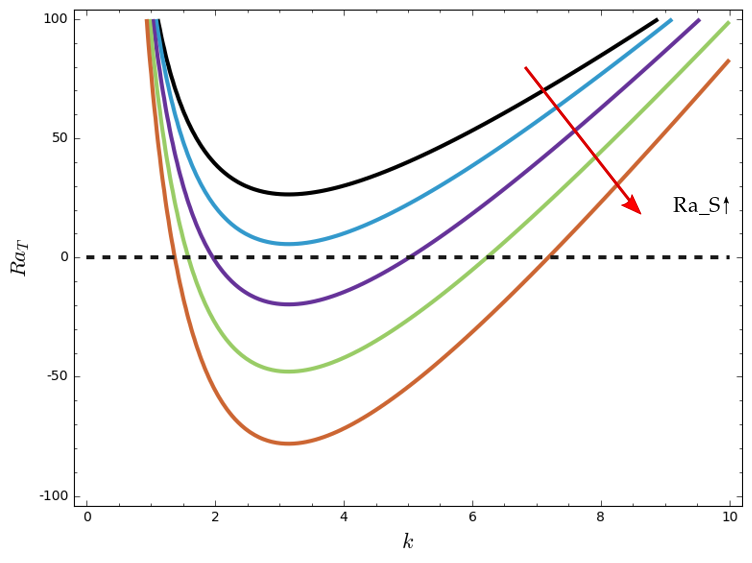
\includegraphics[scale = 0.3]{Figs/energy_stab_Ra_T_vs_k_tau_0_1_vary_Ra_S.png}
    \caption{Marginal energy-stability curve for $\tau = 0.1$, increasing $Ra_{S} = [100, 150, 200, 250, 300]$.}
    \label{fig:energy_stab_Ra_T_vs_k_tau_0_1_vary_Ra_S}
\end{figure}
Finally we compare the energy vs linear stability thresholds.Comparing Eqns.(\ref{eq:lin_marginal_stab}) and (\ref{eq:energy_marginal_stab}), we see that there is a gap between the linear and energy stability thresholds. 
\begin{figure}[H]
    \centering
    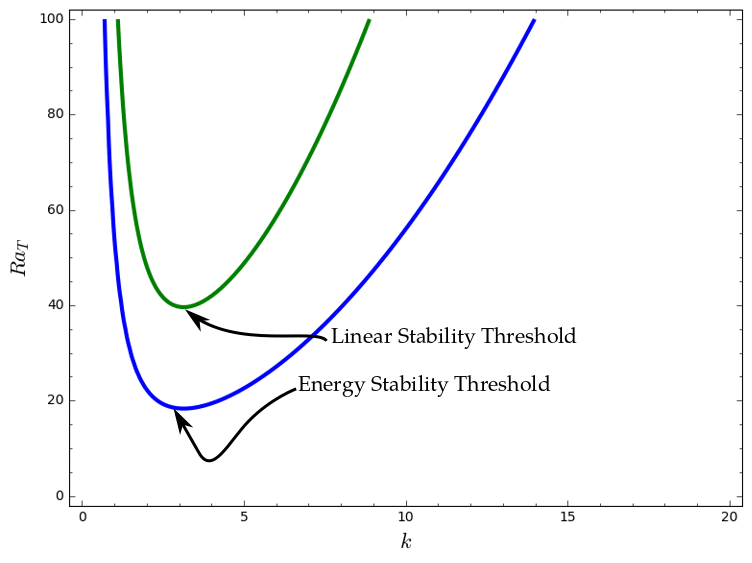
\includegraphics[scale = 0.3]{Figs/lin_vs_energy_stab.png}
    \caption{Comparing linear- vs energy-marginal stability curves. $m = 1$, $Ra_S = 10^{-2}, \tau = 10^{-1}$. We see a clear gap between the thresholds.}
    \label{fig:lin_vs_energy_stab}
\end{figure}

%----------------------------------------
\bibliographystyle{apalike}
%\bibliographystyle{unsrt} % Use for unsorted references  
%\bibliographystyle{plainnat} % use this to have URLs listed in References
%\cleardoublepage
%\bibliography{References/references} % Path to your References.bib file

\bibliography{bib/references} % Path to your References.bib file
 \if@openright\cleardoublepage\else\clearpage\fi
 \cleardoublepage
 \pagestyle{empty}
%--------------------------------------------------------------------
\end{document}
